\label{sec:methods}

This section describes how the research question (Section~\ref{sec:research-question}) was investigated.
We built a simulation platform and ran a sequence of controlled experiments that varied reward terms, action representation (direct torque versus nadir-relative pointing offset), and learning algorithm.
Each configuration was evaluated against the deterministic baseline (Section~\ref{sec:baseline-intro}) under matched environment draws: same altitude, cloud layout, and target positions per episode.
Success is measured by whether the agent learns a stable policy that uses vision feedback to shutter selectively rather than on every step.

The subsections below document every modelling choice, constant, and algorithm in sufficient detail to reproduce the experiment results.
Numeric values appear in the Nomenclature and in the tables below; repository source locations are listed in the Appendix.

% ─────────────────────────────────────────────────────────────────────────────
\subsection{Environment overview}
\label{sec:env-overview}

The mission is a single-satellite nadir-looking Earth-observation overflight.
One episode represents a single contiguous pass over a ground corridor.

\paragraph{Altitude and orbit.}
The simulation uses a 2D orbit-plane model: the satellite moves as a point on a circle whose true anomaly $\theta_\text{orbit}$ advances at the instantaneous circular orbit rate (in a circular orbit, true anomaly equals orbital angle).
Orbital altitude is sampled uniformly from $[\SI{510}{km},\,\SI{570}{km}]$ per episode; all other geometry scales with altitude, so the choice of specific ground track is arbitrary.

\paragraph{Target corridor.}
Fifty observation targets are placed at fixed positions along a ground corridor directly below the orbit plane.
Their angular positions in the orbit plane are computed once at episode initialisation from the sampled altitude.
The specific geographic location of the corridor is irrelevant: the agent only ever sees orbit-plane angles, cloud fractions, and attitude state.

\begin{figure}[htbp]
  \centering
  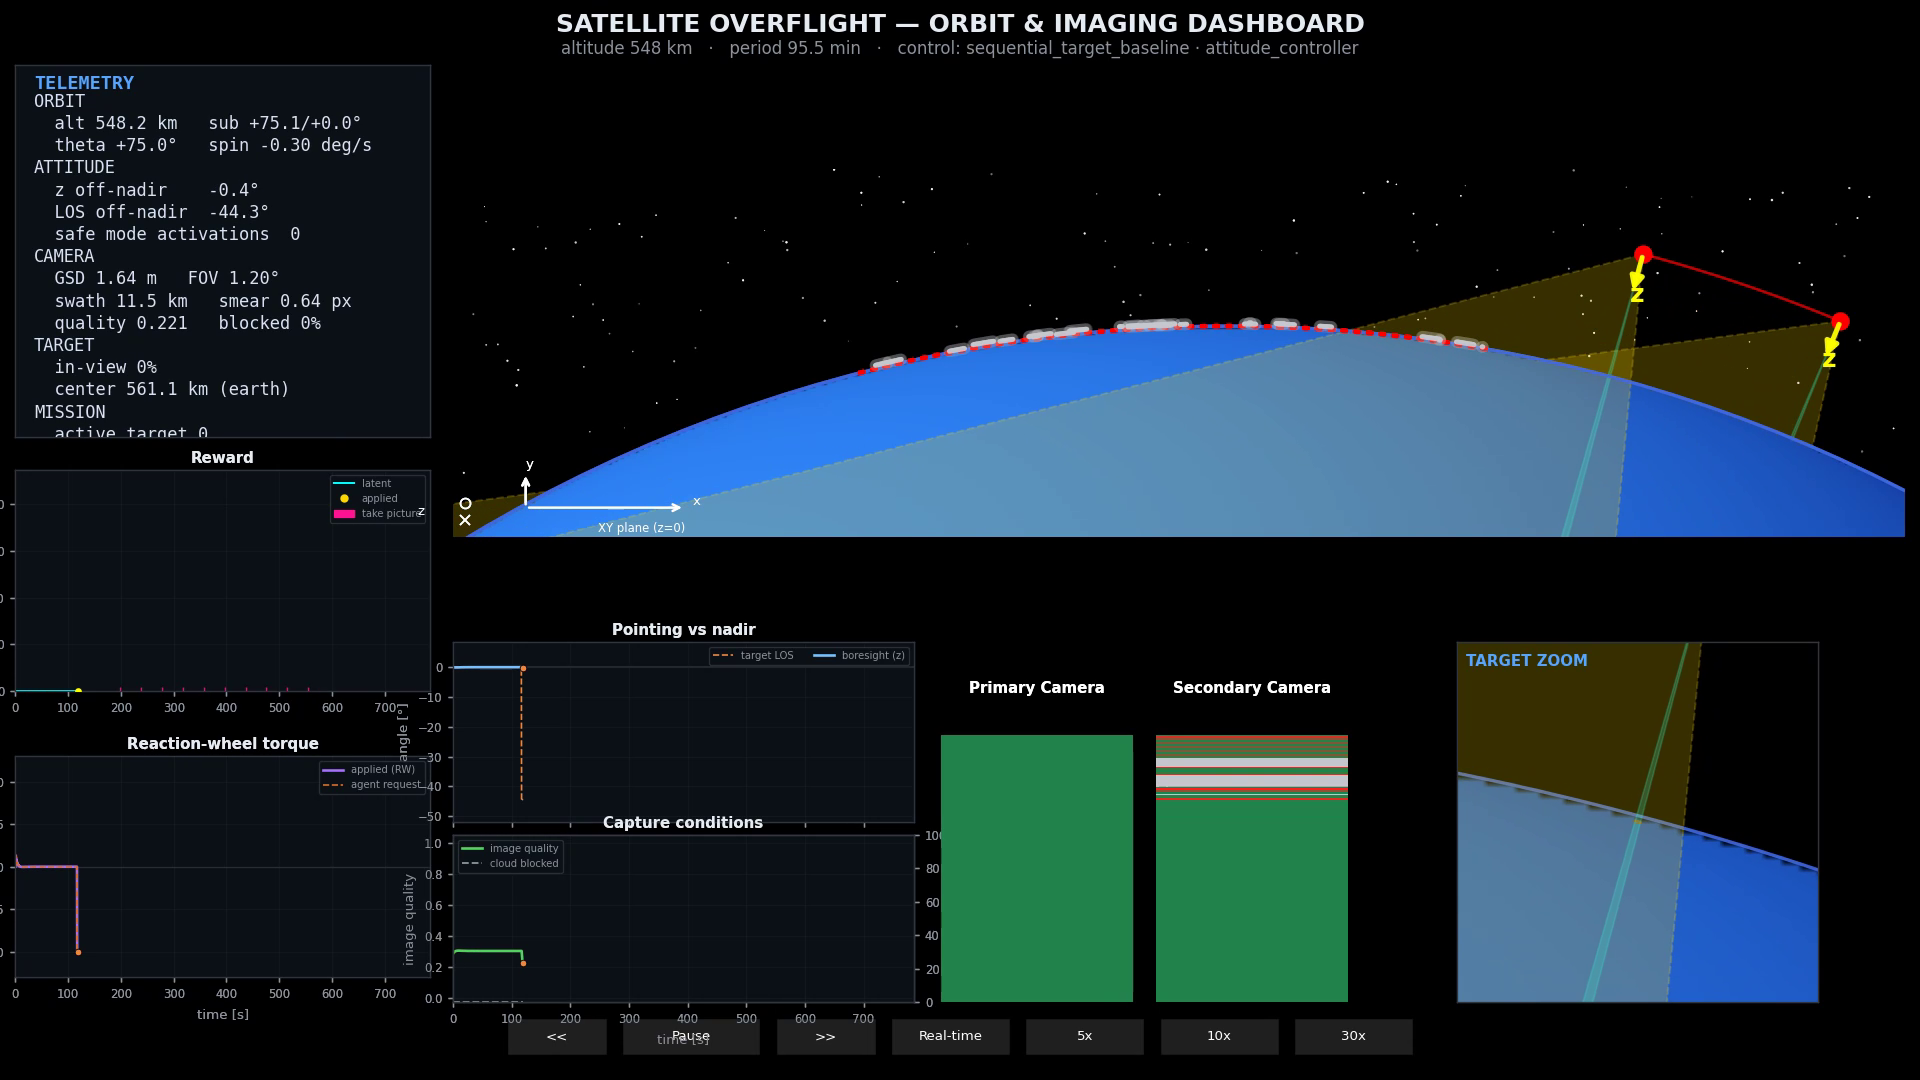
\includegraphics[width=0.92\linewidth]{figures/fig_env_overview.png}
  \caption{Environment overview on the orbit-disk dashboard early in the pass: satellite on the arc, target corridor markers on the Earth limb ahead of the boresight, before the first scheduled slew.}
  \label{fig:env-overview}
\end{figure}

\paragraph{Episode window.}
The episode start and end positions along the pass were tuned so that the first target is not yet visible in the secondary wide-angle camera at episode open, with a small margin at both boundaries.
This trims dead coast time at the corridor edges while keeping the engagement arc inside the pass.
At the canonical simulation timestep of $\Delta t = \SI{1.5}{\second}$ this yields approximately 516 controller steps per episode ($\approx\SI{774}{\second}$).

\paragraph{Off-policy learning and replay buffer.}
\label{sec:replay-buffer}
Training uses two off-policy algorithms, SAC (Section~\ref{sec:sac}) and MPO (Section~\ref{sec:mpo}): the policy is improved from stored past experience, not only from the latest rollout.
After each simulation step the transition (observation, action, reward, next observation) is appended to a \emph{replay buffer}, a fixed-capacity store of recent steps.
Gradient updates draw random mini-batches from this buffer, so a rare rewarded event (a successful capture) can contribute to many parameter updates.
\emph{Capture credit} (the reward applied when a shutter yields a useful first-time observation of a target) is sparse in this environment, so both the simulation timestep below and the warmup protocol in Section~\ref{sec:experiments} affect whether the buffer contains enough useful transitions to learn from.

\paragraph{Simulation timestep selection.}
Choosing $\Delta t$ requires balancing three competing constraints:
\begin{enumerate}
  \item \textbf{Controller authority:} $\Delta t$ must be small enough that the low-level attitude controller can still respond to the reaction-wheel dynamics within one step.
  \item \textbf{Agent decisiveness:} the agent must be able to take meaningful pointing and shutter actions on a timescale relevant to the target encounter windows.
  \item \textbf{Reward signal fidelity:} capture credit arrives only at shutter events on clear targets, so most steps carry little or no reward.
    If $\Delta t$ is too large, target encounters fall between steps and fewer rewarded transitions are stored per episode, leaving the replay buffer (Section~\ref{sec:replay-buffer}) with too little signal for off-policy learning.
\end{enumerate}
To find the largest $\Delta t$ satisfying these constraints we ran a timestep parity sweep over four candidates:
$\Delta t \in \{0.4,\,0.8,\,1.0,\,1.5\}\,\si{s}$, with controller update interval matched to $\Delta t$.
Each candidate ran one baseline warmup episode and had to satisfy: at least one shutter and episode return $\ge 50\%$ of the $\SI{0.4}{s}$ reference.
All four candidates passed.
$\Delta t = \SI{1.5}{\second}$ was selected as the largest parity-passing timestep, cutting the episode from $\sim 1935$ to $\sim 516$ controller steps and proportionally increasing training throughput.

% ─────────────────────────────────────────────────────────────────────────────
\subsection{Simplifications}
\label{sec:simplifications}

Table~\ref{tab:simplifications} summarises which subsystems are modelled and which are deliberately omitted.

\begin{table}[htbp]
  \centering
  \caption{Modelled vs.\ not-modelled subsystems.}
  \label{tab:simplifications}
  \renewcommand{\arraystretch}{1.3}
  \small
  \begin{tabular}{@{}>{\raggedright\arraybackslash}p{0.22\linewidth}>{\raggedright\arraybackslash}p{0.36\linewidth}>{\raggedright\arraybackslash}p{0.34\linewidth}@{}}
    \toprule
    Subsystem & Modelled & Not modelled \\
    \midrule
    Orbit propagation     & Circular 2D (disk model) & $J_2$, atmospheric drag, eclipse \\
    Attitude dynamics     & 2D rigid body, reaction-wheel torque chain & 3-axis, flexibility, RW friction \\
    Camera                & 1D ray tracing, image quality (motion smear) & Radiometric calibration, TDI, MTF \\
    Cloud occlusion       & Parameterised cloud-arc primitives & Spatially correlated fields, multi-layer \\
    Terrain               & Spherical Earth (WGS84 for geodesy only) & DEM, shadow, surface reflectance \\
    Multi-orbit mission   & Single pass per episode & Revisit scheduling, downlink windows \\
    Hardware latency      & Not modelled & Onboard CPU budget, comms delay \\
    \bottomrule
  \end{tabular}
\end{table}

The 2D simplification is the most consequential: all attitude variables are scalar ($\theta_\text{body}$, $\omega_\text{sat}$, $\omega_\text{wheel}$), and out-of-plane dynamics are absent.
This is consistent with the scope stated in the introduction and is a known limitation (Section~\ref{sec:limitations}).

% ─────────────────────────────────────────────────────────────────────────────
\subsection{Dynamics model}
\label{sec:dynamics}

\paragraph{Equations of motion.}
The satellite body angle $\theta_\text{b}$ and inertial rate $\omega_\text{sat}$ evolve under a single-axis reaction-wheel coupling:
\begin{align}
  \dot\omega_\text{sat} &= -\,\frac{\tau_\text{wheel}}{I_\text{sat}}, &
  \dot\omega_\text{wheel} &= \frac{\tau_\text{wheel}}{I_\text{wheel}}, &
  \dot\theta_\text{b} &= \omega_\text{sat},
\end{align}
where $I_\text{sat} = \SI{31.2}{kg.m^2}$ (Table~\ref{tab:constants-earth-spacecraft}) and
the wheel inertia $I_\text{wheel} = \tau_\text{max,RW}/\omega_\text{w,max}= \SI{0.1}{N.m}/\SI{150}{rad.s^{-1}}$.
Both are integrated forward with forward-Euler at $\Delta t_\text{sim} = \SI{1.5}{\second}$ (Table~\ref{tab:constants-camera-sim}).

\paragraph{Reaction-wheel limits.}
The wheel applies a torque $|\tau_\text{wheel}|\le\tau_\text{max,RW}=\SI{0.1}{N.m}$ and
stores angular momentum up to $H_\text{max}=\SI{0.4}{N.m.s}$.
A low-level rate gate blocks commands that would accelerate the satellite body beyond the star-tracker rate limit of $\dot\theta_\text{max}=\SI{3}{\degree.s^{-1}}$; decelerating torques are always passed.

\paragraph{Satellite mass.}
Bus mass is $m_\text{sat}=\SI{250}{kg}$ (relevant only for orbit-speed computation; inertia is the primary dynamics parameter).

% ─────────────────────────────────────────────────────────────────────────────
\subsection{Overflight and observation model}
\label{sec:obs-model}

\paragraph{Camera geometry.}
The primary nadir-looking camera parameters are listed in Table~\ref{tab:constants-camera-sim}.
The vertical field of view and ground-sampling distance (GSD) are computed analytically from sampled altitude using a pinhole model.
At $\SI{540}{km}$ the nominal GSD is approximately $\SI{1.6}{m}$.

\paragraph{Lookahead sensing.}
The secondary camera is a forward-tilted wide-angle (fisheye) imager: $\SI{25}{\degree}$ off nadir in the prograde direction with a $\SI{70}{\degree}$ along-track field of view
(Table~\ref{tab:constants-camera-sim}).
It provides early visibility of upcoming targets and cloud occlusion so the controller can decide among multiple imaging opportunities before they enter the primary nadir footprint (Section~\ref{sec:solution-concept}).

\paragraph{Camera observation lines.}
At each simulation timestep the primary and secondary cameras are evaluated as one-dimensional observation lines spanning their vertical fields of view (Table~\ref{tab:constants-camera-sim}).
Each line reports target coverage and cloud occlusion along the boresight strip; both use the same ray-intersection kernel.

\paragraph{Image quality and motion smear.}
Capturing a useful image requires the boresight ground footprint to remain nearly stationary during
the exposure window.
The full derivation proceeds in three steps: (i) compute the boresight ground velocity $v_\text{bore}$
from orbit and body rates; (ii) convert to a physical ground blur $\delta$ during exposure; (iii) map
$\delta$ to a scalar quality score $q\in[0,1]$.

\subparagraph{Step 1: Boresight ground speed.}
In the 2D orbit-disk model the satellite position is
\begin{equation}
  \vec{s} = r_\text{orb}\,[\cos\theta_\text{orb},\,\sin\theta_\text{orb}]^\top,
\end{equation}
with orbital radius $r_\text{orb}$ and true anomaly $\theta_\text{orb}(t)$ advancing at angular rate
$\dot\theta_\text{orb} = \omega_\text{orb}$.
The boresight unit vector in the disk plane is
\begin{equation}
  \hat{d} = [\cos\phi,\,\sin\phi]^\top,\qquad
  \dot\phi = \omega_\text{body},
\end{equation}
where $\phi$ is the absolute boresight angle (body angle plus nadir direction) and
$\omega_\text{body} = \dot\theta_\text{body}$ is the current body rate.

The boresight ray $\vec{s} + t\,\hat{d}$ intersects the WGS84 oblate spheroid
($a = \SI{6378137}{m}$, $b = \SI{6356752}{m}$) at slant distance $t^\star$ from the
positive root of
\begin{equation}
  A\,t^2 + B\,t + C = 0, \label{eq:ray-ellipsoid}
\end{equation}
where
\begin{align}
  A &= \frac{d_x^2 + d_y^2}{a^2} + \frac{d_z^2}{b^2}, \\
  B &= 2\!\left(\frac{s_x d_x + s_y d_y}{a^2} + \frac{s_z d_z}{b^2}\right), \\
  C &= \frac{s_x^2 + s_y^2}{a^2} + \frac{s_z^2}{b^2} - 1.
\end{align}
(All 3-D coordinates are obtained by embedding the 2D disk in the $(x,z)$ ECEF plane.)

The boresight ground hit is $\vec{g} = \vec{s} + t^\star\,\hat{d}$.
Differentiating implicitly with respect to time:
\begin{equation}
  \dot t^\star = -\,\frac{\dot A\,(t^\star)^2 + \dot B\,t^\star + \dot C}{2A\,t^\star + B},
  \label{eq:tdot}
\end{equation}
where $\dot A$, $\dot B$, $\dot C$ are computed from $\dot{\vec{s}}$ (satellite velocity) and
$\dot{\hat{d}}$ (boresight rotation rate):
\begin{equation}
  \dot{\vec{s}} = r_\text{orb}\,\omega_\text{orb}\,[-\sin\theta_\text{orb},\,0,\,\cos\theta_\text{orb}]^\top,
  \qquad
  \dot{\hat{d}} = \omega_\text{body}\,[-\sin\phi,\,0,\,\cos\phi]^\top.
\end{equation}
The hit velocity is then
\begin{equation}
  \dot{\vec{g}} = \dot{\vec{s}} + \dot t^\star\,\hat{d} + t^\star\,\dot{\hat{d}}.
  \label{eq:gdot}
\end{equation}
The boresight ground speed is $v_\text{bore} = \|\dot{\vec{g}}\|$.

\subparagraph{Step 2: Ground blur during exposure.}
During a finite exposure $t_\text{exp} = \SI{100}{\micro s}$ the boresight footprint moves
\begin{equation}
  \delta = v_\text{bore}\,t_\text{exp}\quad[\si{m}].
\end{equation}
The pixel smear in GSD units is
\begin{equation}
  \sigma = \frac{\delta}{\text{GSD}_\text{eff}},
\end{equation}
where the effective GSD at off-nadir angle $\alpha$ is
$\text{GSD}_\text{eff} = \text{GSD}_0 / \cos\alpha$,
with nadir GSD
\begin{equation}
  \text{GSD}_0 = \frac{p\cdot h}{f} = \frac{\SI{3.2}{\micro m}\cdot h}{\SI{1067}{mm}}
\end{equation}
(pixel pitch $p$, altitude $h$, focal length $f$).
At $h = \SI{540}{km}$: $\text{GSD}_0 \approx \SI{1.62}{m}$,
giving a nadir swath of $9344 \times \SI{1.62}{m} \approx \SI{15.1}{km}$ along-track.

\subparagraph{Step 3: Normalised quality score.}
Rather than using smear in pixels (which depends on altitude), quality is expressed in physical
ground units via a Lorentzian:
\begin{equation}
  q = \frac{r}{\delta + r}, \qquad
  r = \SI{0.30}{m},\quad t_\text{exp} = \SI{100}{\micro s}.
  \label{eq:quality}
\end{equation}
Properties: $q \to 1$ as $\delta \to 0$ (perfect tracking); $q = 0.5$ at $\delta = r = \SI{0.30}{m}$;
$q$ is indifferent to GSD (quality degrades from optical smear, not pixel count).

\subparagraph{Characteristic regimes.}
At the canonical orbit ($h = \SI{540}{km}$, $\omega_\text{orb} \approx \SI{1.08e-3}{rad.s^{-1}}$):
\begin{itemize}
  \item \textbf{Nadir, zero body rate:} $v_\text{bore} = r_\text{orb}\,\omega_\text{orb} \approx \SI{7.6}{km.s^{-1}}$,
    $\delta \approx \SI{0.76}{m}$, $q \approx 0.28$.
  \item \textbf{Target-tracking ($\omega_\text{body} = \omega_\text{orb}$):} $v_\text{bore} \approx 0$,
    $\delta \approx 0$, $q \approx 1.0$.
  \item \textbf{Half-tracking:} $\omega_\text{body} = 0.5\,\omega_\text{orb}$,
    $\delta \approx \SI{0.38}{m}$, $q \approx 0.44$.
\end{itemize}
The quality factor directly enters the capture-credit reward (Eq.~\ref{eq:r-cap}),
giving the agent an incentive to slow the boresight ground motion by pointing toward
and tracking each target across its observation window.

\begin{figure}[htbp]
  \centering
  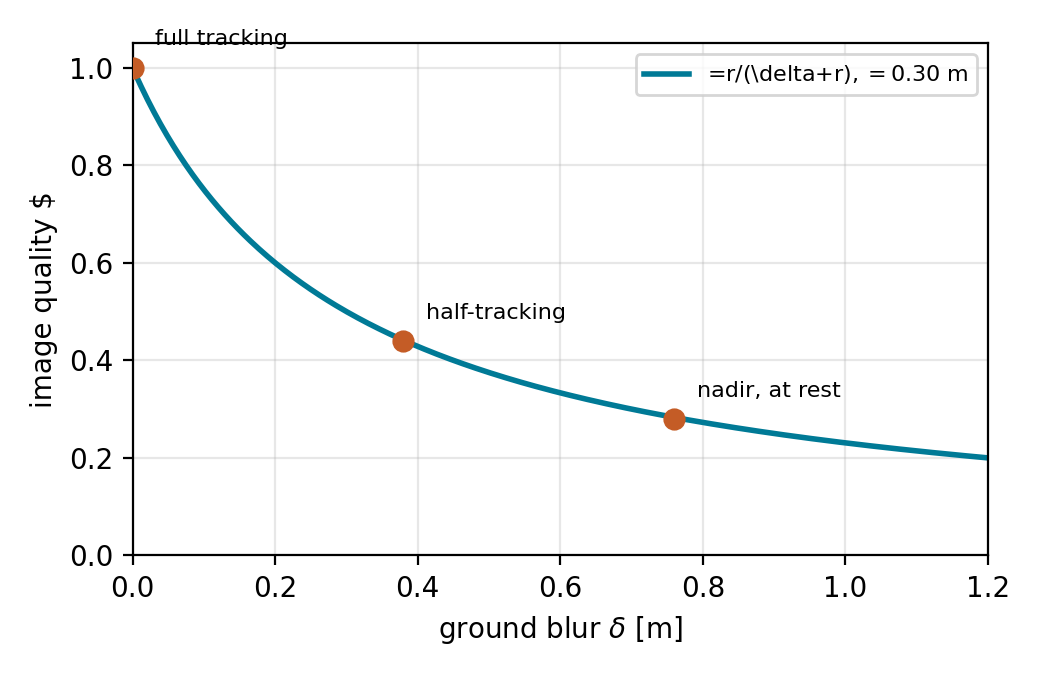
\includegraphics[width=0.72\linewidth]{figures/fig_image_quality_curve.png}
  \caption{Normalised image quality $q=r/(\delta+r)$ with $r=\SI{0.30}{m}$.
    Annotated operating points match the nadir-at-rest, half-tracking, and full-tracking regimes above.}
  \label{fig:image-quality-curve}
\end{figure}

\paragraph{Cloud model.}
Cloud primitives are parameterised arcs in the orbit plane.
For each episode a seeded generator places cloud patches along the target corridor with extent, altitude, and thickness drawn from the ranges in Table~\ref{tab:constants-mission}.
Over a single pass the clouds are effectively fixed relative to the ground corridor (any advective drift is negligible on the episode timescale); occlusion changes mainly because the satellite and camera rays move through that layout.
The cloud-blocked fraction along each camera observation line is computed at every timestep and contributed to the per-step observation and reward.

% ─────────────────────────────────────────────────────────────────────────────
\subsection{Baseline strategy}
\label{sec:baseline}

The reference controller is a deterministic sequential-target overflight policy.
Figure~\ref{fig:baseline-overflight-phases} shows the approach, point, and capture phases of a typical pass; Table~\ref{tab:baseline-config} lists the scheduling logic, OBC PD gains, lock threshold, lead margin, shutter commands, and cloud awareness.
The baseline uses the same attitude-safety stack and simulation kernel as the learned policy: safety overrides are not disabled.

\begin{table}[htbp]
  \centering
  \renewcommand{\arraystretch}{1.3}
  \caption{Deterministic baseline configuration (comparison anchor).}
  \label{tab:baseline-config}
  \small
  \begin{tabular}{p{0.32\linewidth}p{0.62\linewidth}}
    \toprule
    Aspect & Setting \\
    \midrule
    Scheduling logic &
      Strided target list: 10 captures per pass from a 50-target corridor (indices 0, 5, 10, \ldots, 45 on the evaluation seed).
      Nadir coast between engages; slew to target bearing when the orbit-angle window opens. \\
    OBC pointing &
      PD loop on body-angle tracking error; gains $k_p \approx \SI{1.15}{N.m/rad}$, $k_d \approx \SI{12.0}{N.m.s/rad}$
      derived from $\tau_\text{max}=\SI{0.1}{N.m}$, $I_\text{sat}=\SI{31.2}{kg.m^2}$, and a \SI{5}{\degree} deceleration band. \\
    Boresight lock threshold &
      $\SI{15}{\degree}$ between body boresight and target bearing (shutter fires once locked, or if image quality $\ge 0.25$ while the target is in the sensor strip). \\
    Lead margin &
      \SI{20}{\degree} orbit-angle margin before target engage window opens. \\
    Shutter commands &
      10 per episode (one per scheduled target; matches the episode capture cap). \\
    Cloud awareness &
      None (captures on schedule regardless of occlusion). \\
    \bottomrule
  \end{tabular}
\end{table}

In each learning run the same baseline policy fills five warmup episodes under that run's action interface and reward stack;
the mean warmup return is therefore the matched \emph{average baseline return} against which training and evaluation are compared (Section~\ref{sec:exp-table}).

% ─────────────────────────────────────────────────────────────────────────────
\subsection{Attitude safety controller}
\label{sec:safety}

Every torque command, whether from the learned policy or the baseline, passes through the
attitude safety controller before reaching the reaction-wheel plant.
The controller operates in two regimes:

\paragraph{Normal-mode taper.}
In nominal flight the controller applies a linear taper on the commanded torque when the satellite approaches the off-nadir hard limit:
\begin{equation}
  \tau_\text{applied} = \alpha\,\tau_\text{cmd}, \qquad
  \alpha = \mathrm{clip}\!\left(\frac{\theta_\text{hard} - \theta_\text{off-nadir}}{\theta_\text{hard} - \theta_\text{arm}},\,0,\,1\right),
\end{equation}
where $\theta_\text{hard}=\SI{45}{\degree}$ is the hard limit and $\theta_\text{arm}$ is the kinematic braking distance
($\theta_\text{arm}=\theta_\text{hard} - \omega^2/(2\tau_\text{max}/I_\text{sat})$).

\paragraph{Safe-mode entry condition.}
Safe mode is entered when the off-nadir angle equals or exceeds $\theta_\text{hard}$, or when the predicted
overshoot satisfies $\theta_\text{off-nadir} + \theta_\text{brake} \ge \theta_\text{hard}$.

\paragraph{Safe-mode recovery phases.}
Once safe mode is active the agent torque command is replaced by an onboard recovery sequence
(agent commands are ignored throughout):
\begin{enumerate}
  \item \textbf{BRAKE:} zero-rate command until $|\omega_\text{sat}-\omega_\text{orbit}|\le\SI{0.1}{\degree.s^{-1}}$.
  \item \textbf{CRUISE:} slew toward nadir at $\pm\SI{0.35}{\degree.s^{-1}}$ until off-nadir $\le\SI{5.0}{\degree}$.
  \item \textbf{SETTLE:} zero-rate command until off-nadir $\le\SI{1.0}{\degree}$ and rate $\le\SI{0.1}{\degree.s^{-1}}$.
  \item \textbf{LOCKOUT:} hold nadir for $\SI{60}{s}$; agent torque rejected.
\end{enumerate}
After LOCKOUT the controller exits safe mode and normal operation resumes.
All phase thresholds are listed in Table~\ref{tab:safety-thresholds}.

\begin{figure}[htbp]
  \centering
  \begin{subfigure}[t]{0.32\linewidth}
    \centering
    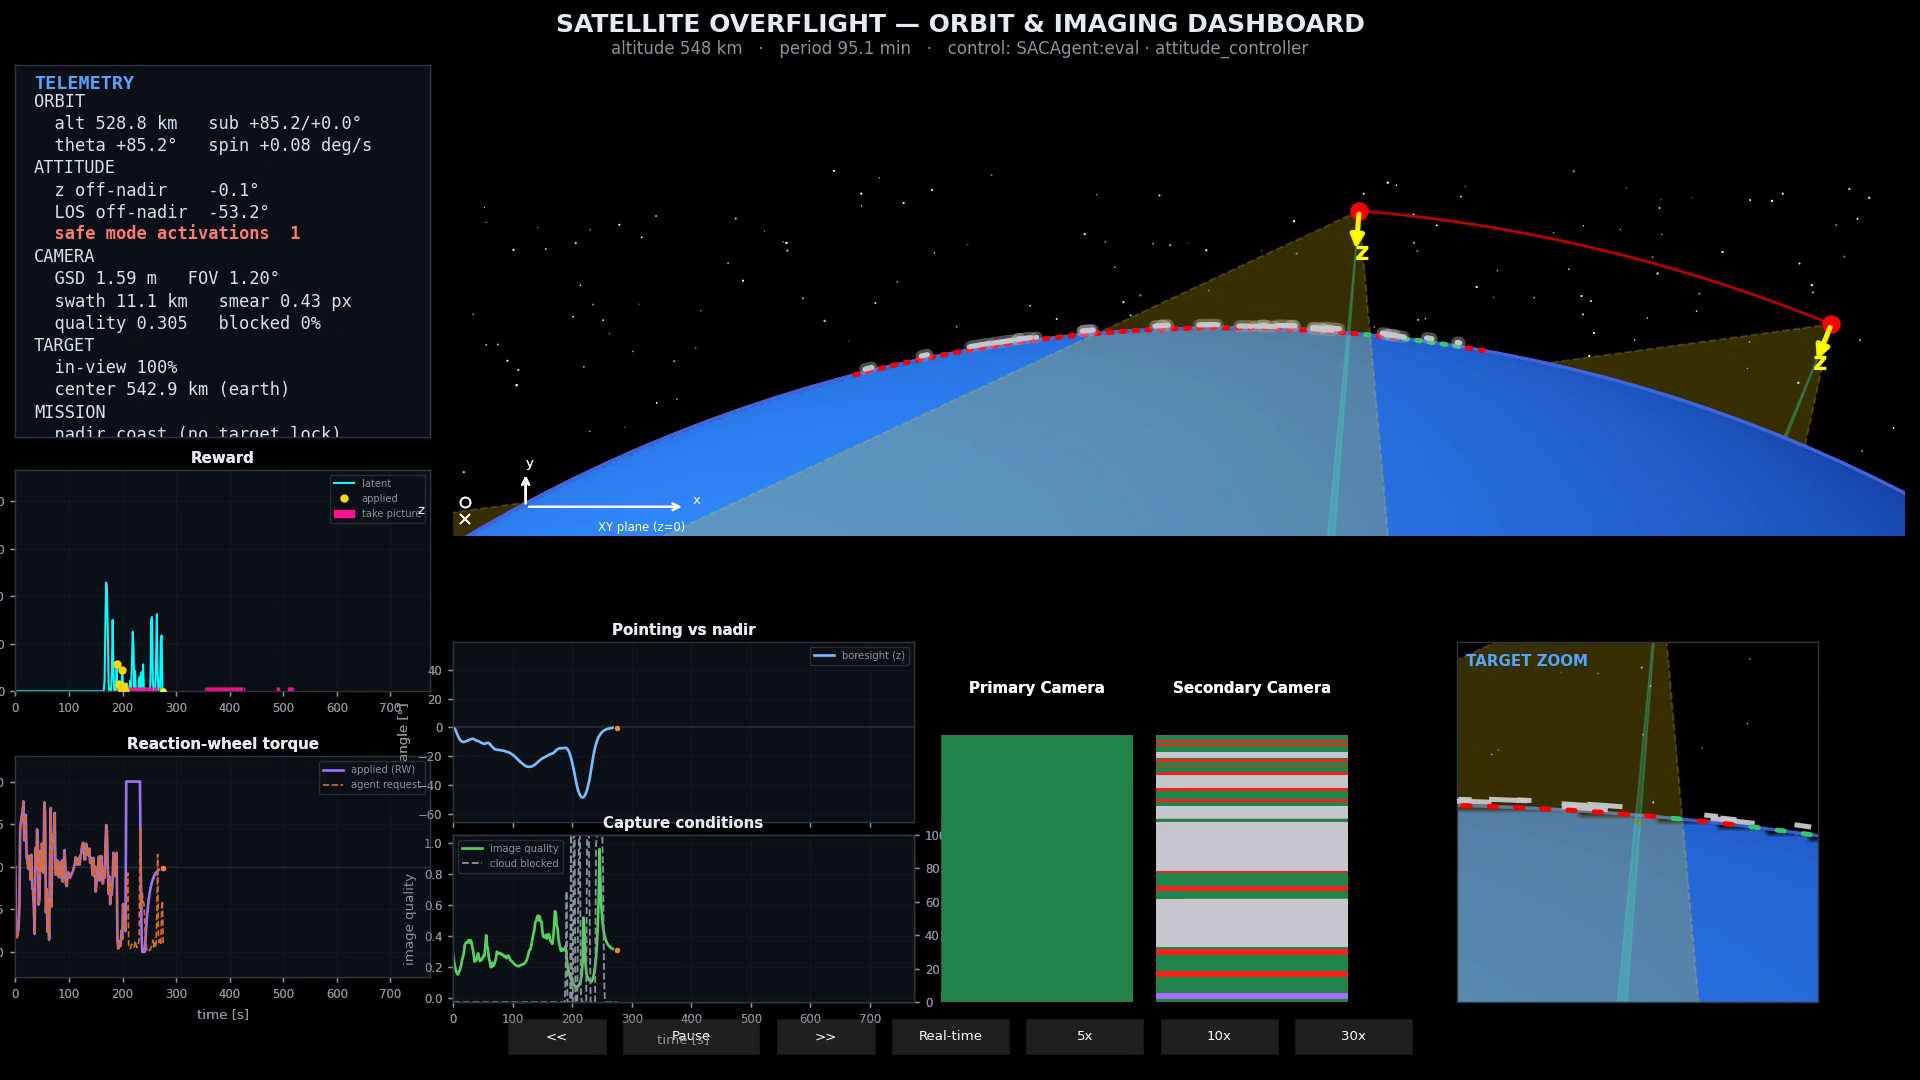
\includegraphics[width=\linewidth]{figures/fig_safety_t0.png}
    \caption{High-torque slew (BRAKE)}
  \end{subfigure}\hfill
  \begin{subfigure}[t]{0.32\linewidth}
    \centering
    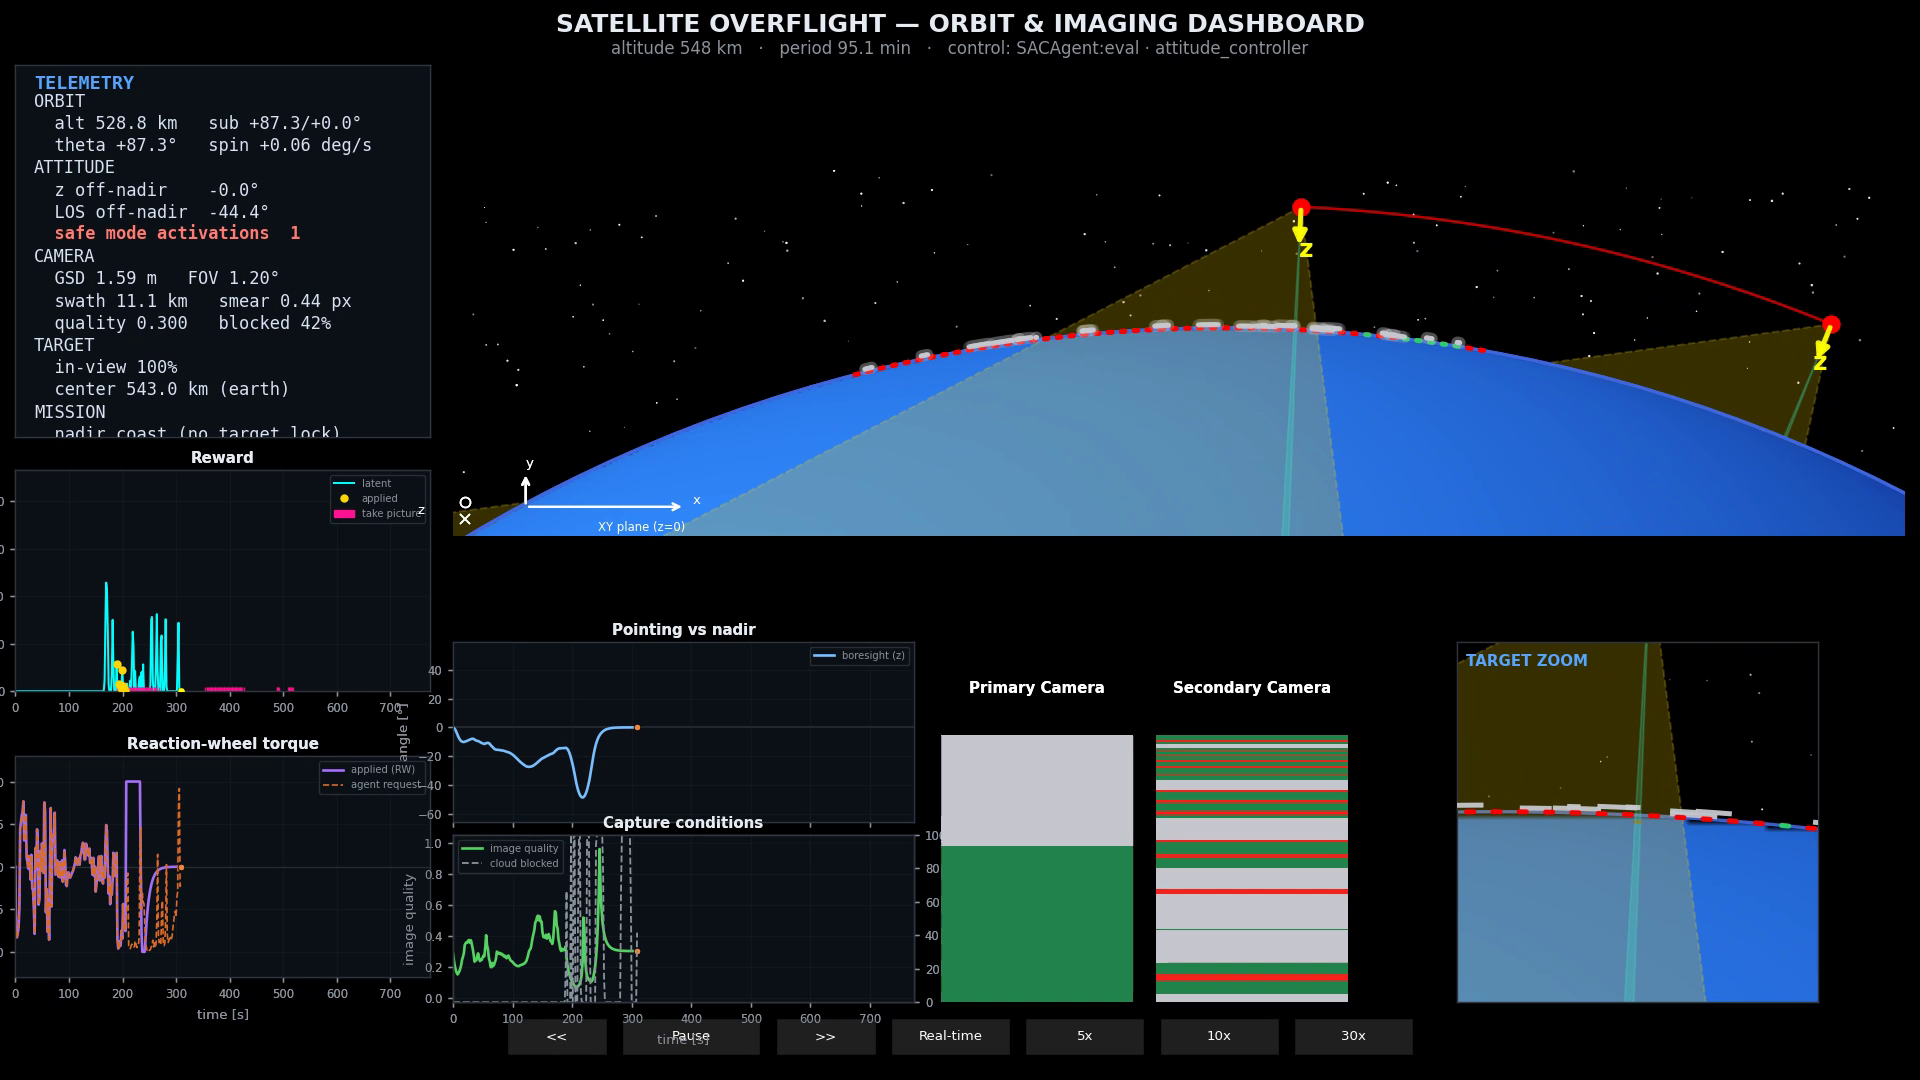
\includegraphics[width=\linewidth]{figures/fig_safety_t1.png}
    \caption{CRUISE}
  \end{subfigure}\hfill
  \begin{subfigure}[t]{0.32\linewidth}
    \centering
    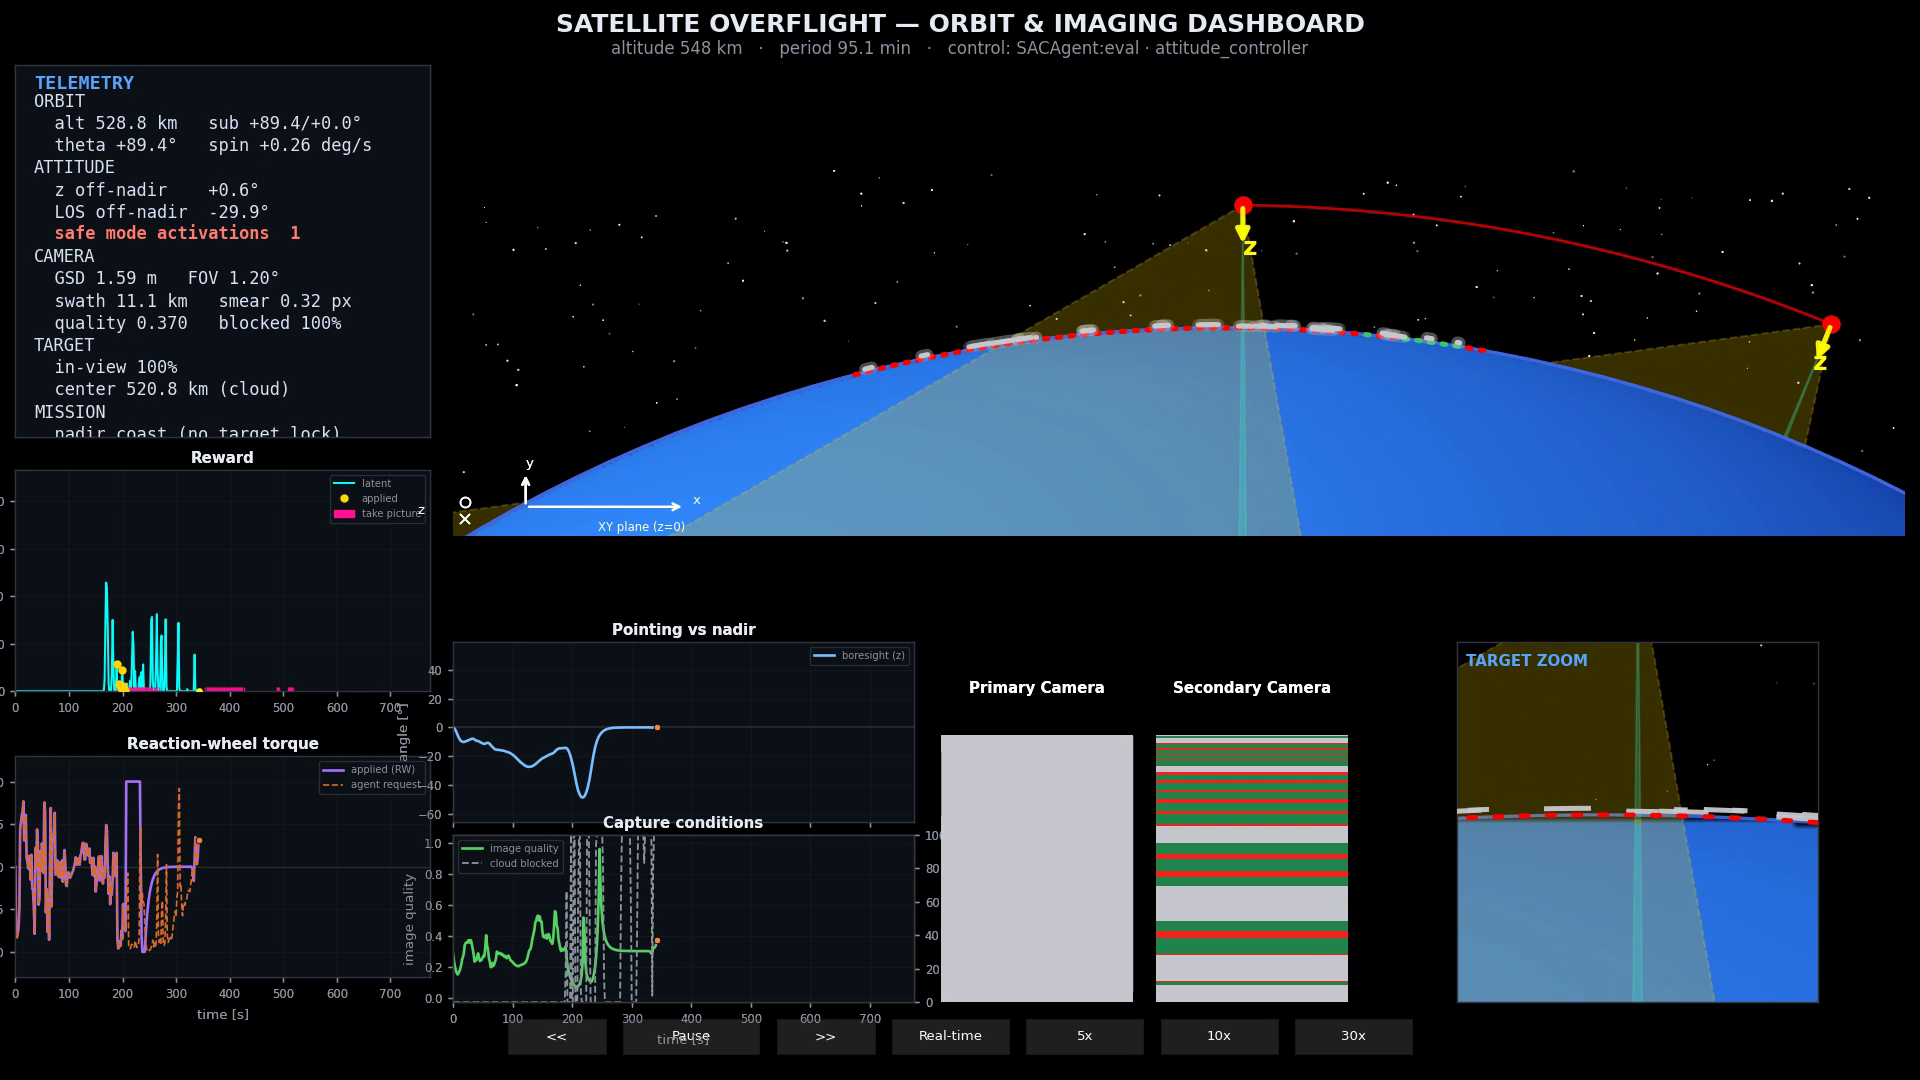
\includegraphics[width=\linewidth]{figures/fig_safety_t2.png}
    \caption{LOCKOUT}
  \end{subfigure}
  \caption{One attitude-safety cycle in torque-mode evaluation (same episode; panels use the recovery-phase names BRAKE / CRUISE / LOCKOUT).
    (a)~High-torque slew: the agent commands large torque and reaches $\approx\SI{43}{\degree}$ off-nadir; safe mode activates (BRAKE) and rejects the request (applied torque drops while the agent request remains high).
    (b)~CRUISE: onboard recovery slews the boresight back toward nadir (here $\approx\SI{24}{\degree}$ off-nadir) while agent torque stays ignored.
    (c)~LOCKOUT: nadir hold with agent torque rejected for $\SI{60}{s}$.
    SETTLE (between CRUISE and LOCKOUT) is short and not shown.}
  \label{fig:safety-maneuver}
\end{figure}

\begin{table}[htbp]
  \centering
  \caption{Attitude safety controller thresholds.}
  \label{tab:safety-thresholds}
  \begin{tabular}{lll}
    \toprule
    Parameter & Symbol & Value \\
    \midrule
    Off-nadir hard limit          & $\theta_\text{hard}$     & $\SI{45}{\degree}$ \\
    Nadir recovery tolerance      & $\theta_\text{tol}$      & $\SI{1.0}{\degree}$ \\
    Decel start (CRUISE$\to$SETTLE) & $\theta_\text{decel}$  & $\SI{5.0}{\degree}$ \\
    Rate stop threshold           & $\omega_\text{stop}$     & $\SI{0.1}{\degree.s^{-1}}$ \\
    Safe-mode cruise rate         & $\dot\theta_\text{crs}$  & $\SI{0.35}{\degree.s^{-1}}$ \\
    Post-recovery lockout         & $t_\text{lock}$          & $\SI{60}{s}$ \\
    \bottomrule
  \end{tabular}
\end{table}

% ─────────────────────────────────────────────────────────────────────────────
\subsection{Reward design}
\label{sec:reward}

The reward is computed per controller step from the full episode simulation state.
All active terms are listed below; inactive terms (distance reward, cloud penalty, energy penalty) were tested in early experiments and disabled by default (see Section~\ref{sec:experiments}).

\paragraph{Capture quality term (applied at shutter events).}
When the agent fires the shutter, is within budget, and the target has not been captured before:
\begin{equation}
  r_\text{cap} = W_\text{cap}\cdot\text{cov}\cdot q\cdot(1 - f_\text{cloud}),
  \label{eq:r-cap}
\end{equation}
where $\text{cov}\in[0,1]$ is the fraction of the primary camera footprint over the dominant target,
$q\in[0,1]$ is the image quality (Section~\ref{sec:obs-model}),
$f_\text{cloud}\in[0,1]$ is the cloud-blocked fraction, and
$W_\text{cap}$ is the capture weight.
Repeat shutters on an already-captured target consume budget but yield zero applied reward.

\paragraph{Budget-exhausted penalty.}
When the agent commands a shutter after the 10-capture budget is exhausted:
$r_\text{budget} = -k_\text{waste}$ with $k_\text{waste}=5.0$ (Exp~7, promoted to default).

\paragraph{Shutter-waste penalty (off by default).}
Optional: when applied capture credit $< \epsilon = 0.001$ on an accepted shutter:
$r_\text{waste} = -k_\text{waste}$. Removed in Exp~9 (see Section~\ref{sec:exp9}).

\paragraph{Torque-effort regulariser (torque mode only).}
\begin{equation}
  r_\text{effort} = -k_\text{eff}\left(\frac{\tau_\text{cmd}}{\tau_\text{max}}\right)^2,
  \qquad k_\text{eff}=0.1.
\end{equation}
Applied every step on the agent-requested torque (before safety arbitration); disabled automatically in vector mode.

\paragraph{Safe-mode penalty (Exp~10 only, not default).}
Per-step penalty while the agent is in safe-mode recovery: $r_\text{safe} = -k_\text{safe}$, $k_\text{safe}=2.0$.
Ruled out at this coefficient (see Section~\ref{sec:exp10}).

% ─────────────────────────────────────────────────────────────────────────────
\subsection{Learning algorithm: SAC}
\label{sec:sac}

We use Soft Actor-Critic (SAC) \cite{haarnoja2018sac}.
SAC is an off-policy actor-critic algorithm in the \emph{maximum-entropy} reinforcement-learning framework:
the stochastic policy maximises expected return while also maximising action entropy, so that high-reward behaviour is learned without collapsing prematurely to a near-deterministic action.
In continuous control, this yields a stable off-policy learner that reuses replay-buffer experience and explores via the entropy term rather than via an additive noise process.

\paragraph{Soft critic update (policy evaluation).}
Two critics $Q_{\theta_1},Q_{\theta_2}$ are trained against a shared soft Bellman target built from the minimum of the target critics (clipped double-Q), with an entropy bonus on the next action:
\begin{equation}
  y = r + \gamma(1-d)\,
  \Bigl(
    \min_{i\in\{1,2\}} Q_{\theta_i'}(s',a')
    - \alpha\,\log\pi_\phi(a'|s')
  \Bigr),
  \label{eq:sac-soft-bellman}
\end{equation}
where $a'\sim\pi_\phi(\cdot|s')$, $d\in\{0,1\}$ marks episode termination, and target networks $Q_{\theta_i'}$ are soft-updated with coefficient $\tau$ (Table~\ref{tab:sac-hparams}).
Each critic is fitted by mean-squared error to $y$.

\paragraph{Policy update (soft actor).}
The Gaussian actor $\pi_\phi$ is updated to maximise soft $Q$ while retaining entropy:
\begin{equation}
  J_\pi(\phi)
  = \mathbb{E}_{s\sim\mathcal{B},\,a\sim\pi_\phi}\!
  \Bigl[
    \alpha\,\log\pi_\phi(a|s)
    - \min_{i\in\{1,2\}} Q_{\theta_i}(s,a)
  \Bigr],
  \label{eq:sac-policy}
\end{equation}
which is minimised by stochastic gradient descent (reparameterised samples; tanh-squashed actions with the standard change-of-variables correction on $\log\pi$).

\paragraph{Fixed entropy temperature.}
The temperature $\alpha$ trades off return against entropy.
We use a fixed coefficient $\alpha=0.2$ (no automatic temperature dual), matching the overnight SAC fork used throughout the experiment series.
This is simpler than the learned-$\alpha$ variant of SAC and was sufficient for the sparse-reward regimes in which SAC first showed a learning signal (Exp~3).

\paragraph{Network architecture.}
Actor and critics use the same 1D-CNN encoder and fully connected widths as MPO (Section~\ref{sec:mpo}): two convolutional layers (kernel size~5, channels $[16,32]$, stride~2, embedding dimension~32), then actor head 90 units and critic heads 140 units.
Hyperparameters are listed in Table~\ref{tab:sac-hparams}.

\begin{table}[htbp]
  \centering
  \caption{SAC hyperparameters (default configuration; all SAC experiments unless noted).}
  \label{tab:sac-hparams}
  \begin{tabular}{lll}
    \toprule
    Parameter & Symbol & Value \\
    \midrule
    Batch size               & $B$               & 256 \\
    Replay buffer            & $|\mathcal{B}|$   & 50\,000 \\
    Discount factor          & $\gamma$          & 0.99 \\
    Target network           & $\tau$            & 0.005 \\
    Actor learning rate      & $\eta_\pi$        & $1.5\times10^{-4}$ \\
    Critic learning rate     & $\eta_Q$          & $4.5\times10^{-4}$ \\
    Entropy temperature      & $\alpha$          & 0.2 (fixed) \\
    Warmup episodes           & ---               & 5 \\
    Training episodes         & ---               & 50 (Exp~2: 7) \\
    Eval episodes             & ---               & 2 \\
    Environment seed          & ---               & 7 \\
    \bottomrule
  \end{tabular}
\end{table}

% ─────────────────────────────────────────────────────────────────────────────
\subsection{Learning algorithm: MPO}
\label{sec:mpo}

We use Maximum a Posteriori Policy Optimisation (MPO) \cite{abdolmaleki2018mpo}.
MPO frames policy improvement as a constrained relative-entropy problem solved by alternating E-step and M-step:

\paragraph{E-step (sample-based policy evaluation).}
$Q^\pi$ targets are regressed from a target critic; the new non-parametric policy distribution
$q^\star(a|s) \propto \pi(a|s)\exp(Q^\pi(s,a)/\eta)$
is derived by solving the dual:
\begin{equation}
  \eta^\star = \arg\min_{\eta>0}\;\eta\,\varepsilon_\eta + \eta\log\mathbb{E}_{\pi}\!\left[\exp\!\left(\frac{Q^\pi(s,a)}{\eta}\right)\right],
  \label{eq:mpo-dual}
\end{equation}
where $\varepsilon_\eta=0.1$ is the KL constraint on the temperature dual.

\paragraph{M-step (policy update with trust region).}
A parametric Gaussian policy $\pi_\theta$ is fitted to $q^\star$ subject to decoupled KL constraints on the mean and variance:
\begin{equation}
  \max_\theta\;\mathbb{E}_{q^\star}\!\left[\log\pi_\theta(a|s)\right]
  \quad\text{s.t.}\quad
  \mathrm{KL}(\bar\pi_\mu\|\pi_{\theta,\mu})\le\varepsilon_\mu,\;
  \mathrm{KL}(\bar\pi_\sigma\|\pi_{\theta,\sigma})\le\varepsilon_\sigma,
\end{equation}
with Lagrange multipliers $\alpha_\mu,\alpha_\sigma$ updated by dual ascent
($\varepsilon_\mu=0.1$, $\varepsilon_\sigma=0.01$; Table~\ref{tab:mpo-hparams}).

\paragraph{Decoupled-KL fix (Exp~8).}
Prior to Exp~8 the implementation used a single coupled KL constraint with a shared multiplier,
which led to KL $\to 0$ (frozen policy) or KL $\to \infty$ (exploding critic) depending on initialisation.
The fix implements separate $\alpha_\mu/\alpha_\sigma$ multipliers as specified in \citet{abdolmaleki2018mpo}.
All MPO experiments from Exp~8 onwards use the corrected implementation.

\paragraph{Network architecture.}
Both actor and critic share a 1D-CNN encoder over the camera observation lines (two convolutional layers, kernel size~5, channels $[16,32]$, stride~2, embedding dimension~32)
followed by fully connected layers (actor: 90 units; critic: 140 units).
Hyperparameters are listed in Table~\ref{tab:mpo-hparams}.

\begin{table}[htbp]
  \centering
  \caption{MPO hyperparameters (default configuration; all experiments unless noted).}
  \label{tab:mpo-hparams}
  \begin{tabular}{lll}
    \toprule
    Parameter & Symbol & Value \\
    \midrule
    Batch size               & $B$               & 256 \\
    Replay buffer            & $|\mathcal{B}|$   & 50\,000 \\
    Discount factor          & $\gamma$          & 0.99 \\
    Target network           & $\tau$            & 0.005 \\
    Actor learning rate      & $\eta_\pi$        & $4.5\times10^{-4}$ \\
    Critic learning rate     & $\eta_Q$          & $1.0\times10^{-3}$ \\
    Dual learning rate       & $\eta_\eta$       & $1.0\times10^{-3}$ \\
    KL samples (E-step Q)    & $N_Q$             & 80 \\
    KL samples (M-step)      & $N_\pi$           & 40 \\
    KL temperature constraint & $\varepsilon_\eta$ & 0.1 \\
    KL mean constraint        & $\varepsilon_\mu$  & 0.1 \\
    KL variance constraint    & $\varepsilon_\sigma$& 0.01 \\
    Warmup episodes           & ---               & 5 \\
    Training episodes         & ---               & 50 (except Exp~14: 350) \\
    Eval episodes             & ---               & 2 \\
    Environment seed          & ---               & 7 (Exps~1--13) \\
    \bottomrule
  \end{tabular}
\end{table}

% ─────────────────────────────────────────────────────────────────────────────
\subsection{Observation and action space}
\label{sec:obs-action}

\paragraph{Observations.}
The controller observation is assembled at each controller tick from:
\begin{itemize}
  \item \textbf{Attitude scalars:} body angle $\theta_\text{body}$ [rad], satellite body rate $\omega_\text{sat}$ [rad/s].
  \item \textbf{Orbit scalar:} true anomaly $\theta_\text{orbit}$ [rad].
  \item \textbf{Camera lines:} primary and secondary observation-line arrays (per-cell class labels: background, target identity, or cloud-blocked).
  \item \textbf{Mission context:} remaining shutter budget (dimensionless count); binary target-captured mask (one entry per target area); signed bearing error toward each target [rad].
\end{itemize}

\paragraph{Actions.}
Both SAC and MPO policies output a 2-dimensional continuous action $[a_\tau, a_s]\in[-1,1]^2$:
\begin{itemize}
  \item \textbf{Torque mode:} $a_\tau\mapsto\tau_\text{cmd} = a_\tau\cdot\tau_\text{max}$ [\si{N.m}] (direct RW torque request).
  \item \textbf{Vector mode:} $a_\tau\mapsto f_n = \SI{45}{\degree}\cdot a_\tau$ (nadir-relative pointing offset); the OBC PD controller converts this to a torque command.
  \item \textbf{Shutter:} $a_s\mapsto (a_s+1)/2\in[0,1]$; boolean shutter command when mapped value $> 0.5$.
\end{itemize}
The torque versus vector mode is a configuration choice at training time;
experiments from Exp~11 onward use vector mode as the default.

% ─────────────────────────────────────────────────────────────────────────────
\subsection{Simulation architecture}
\label{sec:arch}

Training, evaluation, and visualisation share one simulated episode per roll-out.
The reward, the evaluation KPIs, and the exported videos therefore reflect the same altitude, cloud layout, attitude trajectory, and camera observations.
Mission randomisation is controlled by a fixed integer seed so that the deterministic baseline and each learned configuration are compared under identical environment draws.
